\chapter{Экспериментальное оценивание характеристик распознавания предложенных алгоритмов и методов} \label{chapt3}

\section{Результаты исследования статистических свойств речевых команд} \label{sect3_1}

\subsection{Описание тестовой базы речевых данных} \label{sect3_1_1}

Для проведения тестирования алгоритмов, предложенных в предыдущей главе, необходимы различные наборы записей.
Главной целью данной работы являлось создание алгоритмов для распознавания речевых команд в кабине пилота самолёта.
Поэтому основной задачей является распознавание ограниченного числа команд в виде слов или в виде фраз в условиях шума.
Но, при этом, возможно проводить проверку алгоритмов и в более простых условиях, например, в условиях без шума или на словаре уменьшенного размера.

По указанным причинам, в работе использовалось несколько наборов записей:
\begin{itemize}
	\item записи 3 слов без шума: имеется 13 дикторов, для каждого из которых записано около 50 реализаций каждого слова;
	\item записи 3 слов с шумом в наушниках: имеется 4 диктора, которые сделали записи в различных вариантах шума в наушниках (без шума, с шумом 80 дБ и с шумом 90 дБ), в каждом из вариантов записано по 53 реализации каждого слова;
	\item записи 3 слов с шумом с обратной связью: имеется 4 диктора, для каждого из которых записано по 53 реализации каждого слова;
	\item записи 20 слов без шума: имеется 10 дикторов, для каждого из которых записано по 30 реализации каждого слова;
	\item записи 11 фраз без шума: имеется 7 дикторов, для каждого из которых записано по 30 реализаций каждой фразы, также имеется по 30 записей каждой фразы, которые произносятся разными дикторами --- каждый диктор произносит каждую из фраз не более 2 раз;
	\item записи шума в кабине пилота, длина записи составляет несколько часов, что позволяет накладывать уникальные участки шума на каждую из реализаций, также отдельная запись шума позволяет варьировать отношение сигнал/шум и проверять зависимость качества распознавания в зависимости от этого отношения.
\end{itemize}

В качестве речевых команд для распознавания использовались слова и фразы, наиболее часто используемые в качестве управляющих команд в кабине пилота:
\begin{itemize}
	\item 3 слова: \textsc{пилотаж, масштаб, навигация};
	\item 20 слов: \textsc{пилотаж, масштаб, навигация, тысяча, меньше, два, двадцать, взлёт, пятьсот, ноль, двести, сто, десять, пять, пятьдесят, посадка, больше, руление, один, маршрут};
	\item 11 фраз: \textsc{масштаб меньше, пилотаж масштаб десять, масштаб пилотаж сто, пилотаж масштаб двести, масштаб пилотаж двести, навигация масштаб пятьдесят, навигация масштаб полторы тысячи, масштаб двадцать, масштаб пятьдесят, масштаб тысяча пятьсот, масштаб больше}.
\end{itemize}

Шум в наушниках реализуется следующим образом.
Наушники, в которые поступает шум с заданной громкостью, надеваются диктором, после чего ему тяжело услышать свой голос.
Это используется для того, чтобы в экспериментальных условиях проверить степень изменения речи диктора в зависимости от уровня шума.
Шум лишь поступает в наушники, а не записывается совместно с произносимыми словами.
Это сделано для того, чтобы оценить влияние шума на изменение речи диктора и на процесс распознавания.

Во всех экспериментах данной главы применялось разбиение параметрических портретов на 48 временных отрезков и на 35 частотных полос.
Длительность каждого временного отрезка при таком разбиении равнялась приблизительно 10 мс.
Результаты прошлых исследований показывают, что именно такое разбиение является оптимальным для распознавания через сравнение с эталоном \cite{ilnara2014optimization}.

%\newpage
%============================================================================================================================

\subsection{Результаты оценки характеристик слов} \label{sect3_1_2}

В данном подразделе проведена эмпирическая проверка гипотез о нормальности распределения отклонения элементов параметрических портретов слов от эталона.
Проверяемая гипотеза описана в подразделе \ref{sect2_1_1}.
Также показаны результаты расчётов длительности слов, их энергии и частоты, определённых в подразделе \ref{sect2_1_3}.
Для проверки был использован первый набор данных состоящий из записей 3 слов без шума.
Результаты проверки характеристик всех слов были близки, поэтому для компактности результаты приведены только для одного из слов.
В таблицах \ref{tab:wordCharacteristics} и \ref{tab:wordCharacteristicsAfterSmoothing} приведены оценки основных, описанных в подразделе \ref{sect2_1_3} характеристик для слова <<масштаб>>: длительности сигнала, энергии и частоты.

Используемые в таблицах обозначения:
\begin{itemize}
	\item $\mu(t)$ --- среднее время сигнала в секундах;
	\item $\sigma(t)$ --- среднеквадратическое отклонение времени сигнала в секундах;
	\item $\mu(E) \cdot 10^3$ --- средняя энергия сигнала, помноженная на $10^3$;
	\item $\sigma(E) \cdot 10^3$ --- среднеквадратическое отклонение энергии сигнала, помноженное на $10^3$;
	\item $\mu(\nu)$ --- средняя частота в герцах;
	\item $\sigma(\nu)$ --- среднеквадратическое отклонение сигнала в герцах;
	\item <<доля $H_0$>> --- процент записей слов соответствующего диктора, для которых, в соответствии с критерием Пирсона, принимается гипотеза $H_0$ о нормальности с 5~\% уровнем значимости.
\end{itemize}

В таблице \ref{tab:wordCharacteristics} представлены результаты анализа исходных записей, до выравнивания по амплитуде.

\begin{table}[h]
	\centering
	\caption{Характеристики слова <<масштаб>> до выравнивания по амплитуде}
	\label{tab:wordCharacteristics}
	{\normalsize
		\begin{tabular}{| l | c | c | c | c | c | c | c |}
			\hline
			Диктор & \phantom{0} $\mu(t)$ \phantom{0} & \phantom{0}$\sigma(t)$\phantom{0} & $\mu(E) \cdot 10^3$ & $\sigma(E) \cdot 10^3$ & \phantom{0}$\mu(\nu)$\phantom{0} & \phantom{0}$\sigma(\nu)$\phantom{0} & Доля $H_0$ \\
			\hline
			Г-ов & 0.77	& 0.043 & 1.92 & 0.768 & 686  & 34  & 23~\% \\
			Н-ов & 0.67	& 0.034	& 1.66 & 0.335 & 641  & 396 & 27~\% \\
			Б-ак & 0.67	& 0.023	& 3.80 & 0.898 & 680  & 34  & 36~\% \\
			Ф-ев & 0.67	& 0.023	& 3.80 & 0.898 & 680  & 34  & 36~\% \\
			С-ев & 0.66	& 0.077	& 5.07 & 2.570 & 285  & 305 & 5~\% \\
			Б-як & 0.62	& 0.032	& 0.20 & 0.049 & 805  & 380 & 39~\% \\
			Д-ий & 0.63	& 0.031	& 1.06 & 0.287 & 3177 & 221 & 57~\% \\
			К-ов & 0.68	& 0.052	& 0.50 & 0.163 & 533  & 214 & 39~\% \\
			О-ин & 0.58	& 0.064	& 1.85 & 2.390 & 106  & 125 & 16~\% \\
			С-ов & 0.78	& 0.034	& 2.62 & 1.146 & 1816 & 915 & 43~\% \\
			Т-ов & 0.61	& 0.029	& 0.56 & 0.115 & 590  & 182 & 20~\% \\
			Ц-ин & 0.84	& 0.050	& 0.07 & 0.039 & 1710 & 594 & 25~\% \\
			\hline
		\end{tabular}
	}
\end{table}

В таблице \ref{tab:wordCharacteristicsAfterSmoothing} представлены результаты анализа обработанных записей, после проведение процедуры выравнивания по амплитуде, предложенной в подразделе \ref{sect2_1_2}.

\begin{table}[h]
	\centering
	\caption{Характеристики слова <<масштаб>> после выравнивания по амплитуде}
	\label{tab:wordCharacteristicsAfterSmoothing}
	{\normalsize
		\begin{tabular}{| l | c | c | c | c | c | c | c |}
			\hline
			Диктор & \phantom{0} $\mu(t)$ \phantom{0} & \phantom{0}$\sigma(t)$\phantom{0} & $\mu(E) \cdot 10^3$ & $\sigma(E) \cdot 10^3$ & \phantom{0}$\mu(\nu)$\phantom{0} & \phantom{0}$\sigma(\nu)$\phantom{0} & Доля $H_0$ \\
			\hline
			Г-ов & 0.77	& 0.043 & 1.92 & 3.5E-14 & 686  & 34  & 86~\% \\
			Н-ов & 0.67	& 0.034	& 1.66 & 1.8E-14 & 641  & 396 & 95~\% \\
			Б-ак & 0.67	& 0.023	& 3.80 & 7.4E-15 & 680  & 34  & 66~\% \\
			Ф-ев & 0.67	& 0.023	& 3.80 & 3.4E-14 & 680  & 34  & 95~\% \\
			С-ев & 0.66	& 0.077	& 5.07 & 7.1E-14 & 285  & 305 & 95~\% \\
			Б-як & 0.62	& 0.032	& 0.20 & 3.3E-15 & 805  & 380 & 98~\% \\
			Д-ий & 0.63	& 0.031	& 1.06 & 2.2E-14 & 3177 & 221 & 61~\% \\
			К-ов & 0.68	& 0.052	& 0.50 & 7.7E-15 & 533  & 214 & 82~\% \\
			О-ин & 0.58	& 0.064	& 1.85 & 6.3E-14 & 106  & 125 & 77~\% \\
			С-ов & 0.78	& 0.034	& 2.62 & 5.4E-14 & 1816 & 915 & 86~\% \\
			Т-ов & 0.61	& 0.029	& 0.56 & 1.0E-14 & 590  & 182 & 95~\% \\
			Ц-ин & 0.84	& 0.050	& 0.07 & 2.7E-15 & 1710 & 594 & 93~\% \\
			\hline
		\end{tabular}
	}
\end{table}

Экспериментальные результаты, представленные в таблицах, показывают, что разброс доли проверок, подтверждающих нормальность, составляет от 5 до 57~\% для случая некорректированных по амплитуде слов, и от 60 до 98~\% для слов, корректированных по амплитуде.
Или, другими словами, в среднем, происходит увеличение доли с 30 до 86~\% проверок, подтверждающих нормальность по критерию Пирсона.
Также значительно уменьшился разброс энергии слова относительно среднего значения. 

На рисунке \ref{fig:words_scale} представлены спектрограммы двух дикторов - Д-ий (сверху) и О-ин (снизу).
По горизонтали рисунка обозначена временная ось, выраженная в секундах, а по вертикали --- частота в кГц.
Цвет обозначает уровень энергии на конкретной частоте, энергия возрастает от синего к красному цвету.

\begin{figure}[h]
	\centering
	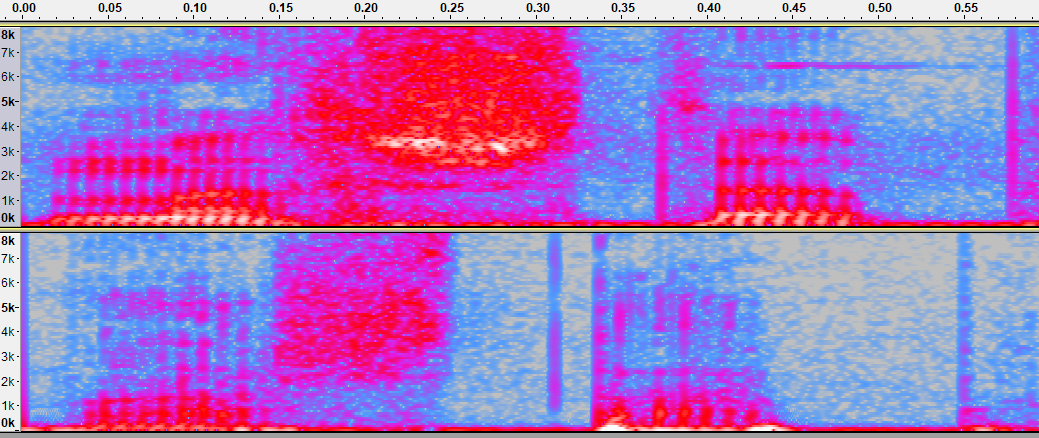
\includegraphics[width=1.0\textwidth]{words_scale.png}
	\caption{Спектрограммы слова <<масштаб>> для дикторов Д-ий (сверху) и О-ин (снизу)}
	\label{fig:words_scale}
\end{figure}

Этот рисунок иллюстрирует различие средней частоты для двух дикторов.
Исходя из полученных результатов, на записи диктора Д-ий наблюдается самое высокое значение средней частоты --- 3177 Гц, в то время как у диктора О-ин зафиксировано самое низкое значение средней частоты --- 106 Гц.
Это означает, что у диктора Д-ий по сравнению с диктором О-ин мало энергии сконцентрировано на низких частотах и много на высоких, или, другими словами, верхняя часть графика более красная, чем другого диктора.
Также это означает, что у диктора О-ин самый низкий голос из представленных дикторов, а у диктора Д-ий --- самый высокий.

Более того, стоит отметить, что частота голоса является довольно стабильной характеристикой диктора, так как её стандартное отклонение $\sigma(\nu)$ мало по сравнению со средним значением $\mu(\nu)$.
Из этого можно сделать вывод, что средняя частота является информативным показателем речи для отдельного человека.
Это свойство может быть использовано для идентификации дикторов по речи.

По результатам статистической проверки можно сделать вывод, что после выравнивания слов по амплитуде входной сигнал удовлетворяет критерию нормальности.
Поэтому дальнейшее использование алгоритмов, требующих нормальности входных данных, обосновано.

%\newpage
%============================================================================================================================

\section{Результаты проверки работоспособности алгоритма разделения слов на однородные части} \label{sect3_2}

В данном подразделе приведены эмпирические результаты работы алгоритма, описанного в подразделе \ref{sect2_2}.
Сутью эксперимента было разбиение нескольких слов на однородные части.
В качестве эталона использовались данные о границах частей, полученные экспертом посредством оценки спектрограмм записи слов с помощью визуального анализа.
Число частей и априорные положения границ, достаточно сильно отличающиеся от эталонных, заданы в качестве исходных условий.
Изначально были предприняты попытки получить численный результат задачи по оптимизации методом перебора.
Это было обусловлено его возможностью находить глобальный экстремум в том случае, если он присутствует в исследуемой области поиска.
Но в таком случае ожидаемой проблемой является ограничение вычислительной мощности современных вычислительных машин, ввиду которой время вычисления результатов увеличивается до нескольких часов при большом количестве частей.
Поэтому было продемонстрировано несколько примеров сравнения метода перебора и алгоритмов динамического программирования, представленных выше.
В ходе сравнения была установлена высокая степень сходства полученных результатов.
Ввиду чего далее был применён подход динамического программирования, способный разделять записи каждого слова на однородные части не более чем за 1 секунду.

Изучались записи команд в виде слов, длительность произнесения которых равна 0.5--1 с, а размер каждого элементарного интервала постоянный и равняется 10 мс.
В результате, разделение команд осуществлялось на 50--100 элементарных интервалов.
Частота регистрации для используемых записей была равна 22050 Гц.
Было рассмотрено разбиение слова на 3--7 частей, каждая из которых могла включать в себя от 2 до 25 интервалов.
Интервал возможного приращения границ частей находится в пределах от минус 5 до плюс 5 элементарных интервалов от изначального местонахождения границ.
Каждое слово было обработано несколько раз для различных априорных данных по расположению границ.
При этом практически отсутствовала зависимость результатов от априорных оценок при условии, что оптимальное значение находилось в области поиска.

На рисунке \ref{fig:word_1000} и в таблице \ref{tab:results_1000} отображены способы разделения слова <<тысяча>> экспертным путём и автоматическим алгоритмом.
Слово <<тысяча>> позволяет выделить 6 звуков, хорошо различимых на слух, для каждой из его букв.

\begin{figure}[h]
	\centering
	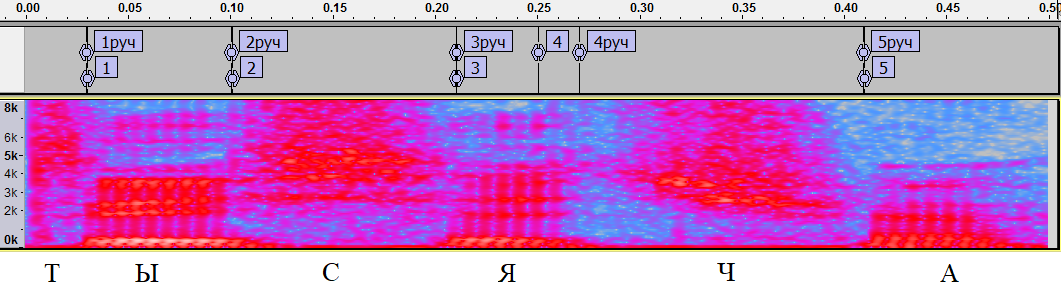
\includegraphics[width=1.0\textwidth]{word_1000.png}
	\caption{Спектрограмма слова <<тысяча>>}
	\label{fig:word_1000}
\end{figure}

\begin{table}[h]
	\centering
	\caption{Границы частей для разных критериев, слово <<тысяча>>}
	\label{tab:results_1000}
	\begin{tabular}{| l | c | c | c | c | c | c |}
		\hline
		\multirow{2}{*}{Функционал} & \multicolumn{5}{c|}{Границы частей, с} & Значение \\
		\hhline{~-----~} & \phantom{00} 1 \phantom{00} & \phantom{00} 2 \phantom{00} & \phantom{00} 3 \phantom{00} & \phantom{00} 4 \phantom{00} & \phantom{00} 5 \phantom{00} & \phantom{00}функционала\phantom{00} \\
		\hline
		$J_{1}$		& 0.03 & 0.10 & 0.21 & 0.25 & 0.41 & 0.75 \\
		$J_{2}$		& 0.03 & 0.10 & 0.21 & 0.24 & 0.41 & 0.01 \\
		$J_{3}$		& 0.03 & 0.10 & 0.21 & 0.25 & 0.41 & 0.13 \\
		$J_{12}$	& 0.03 & 0.10 & 0.21 & 0.24 & 0.41 & 0.74 \\
		$J_{123}$	& 0.03 & 0.10 & 0.21 & 0.24 & 0.41 & 0.60 \\
		\hline
		Вручную		& 0.03 & 0.10 & 0.21 & 0.27 & 0.41 & --- \\
		\hline
	\end{tabular}
\end{table}

Ручное и автоматическое разбиения слова <<больше>> показаны на рисунке \ref{fig:word_more} и представлены в таблице \ref{tab:results_more}.

\begin{figure}[h]
	\centering
 	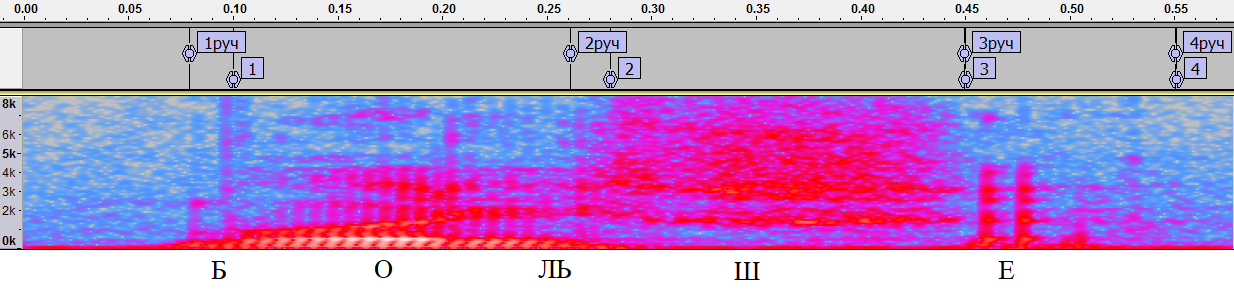
\includegraphics[width=1.0\textwidth]{word_more.png}
	\caption{Спектрограмма слова <<больше>>}
	\label{fig:word_more}
\end{figure}

\begin{table}[h]
	\centering
	\caption{Границы частей для разных критериев, слово <<больше>>}
	\label{tab:results_more}
	{\normalsize
		\begin{tabular}{| l | c | c | c | c | c | c | c | c | c | c | c |}
			\hline
			\multirow{2}{*}{Функционал} & \multicolumn{4}{c|}{Границы частей, с} & Значение \\
			\hhline{~----~} & \phantom{000} 1 \phantom{000} & \phantom{000} 2 \phantom{000} & \phantom{000} 3 \phantom{000} & \phantom{000} 4 \phantom{000} & \phantom{00}функционала\phantom{00} \\
			\hline
			$J_{1}$		& 0.10 & 0.28 & 0.45 & 0.55 & 0.54 \\
			$J_{2}$		& 0.07 & 0.28 & 0.34 & 0.37 & 0.03 \\
			$J_{3}$		& 0.10 & 0.28 & 0.45 & 0.55 & 0.15 \\
			$J_{12}$	& 0.08 & 0.28 & 0.37 & 0.55 & 0.43 \\
			$J_{123}$	& 0.08 & 0.28 & 0.38 & 0.55 & 0.27 \\
			\hline
			Вручную		& 0.08 & 0.26 & 0.45 & 0.55 & --- \\
			\hline
		\end{tabular}
	}
\end{table}

В этом слове первая часть содержит слог <<боль>>, вторая часть --- звук <<ш>> и последняя часть --- звук <<е>>.
Ввиду того, что алгоритм предназначен для нахождения однородных частей, слог <<боль>> полностью относится к первой выделенной части.
Обусловлено это тем, что маленькая длительность звука <<б>> не позволяет выделить его в отдельную часть, а звуки <<о>> и <<ль>> схожи друг с другом \cite{cooper1952some, blumstein1980perceptual}.

Ручное и автоматическое разбиения слова <<двадцать>> показаны на рисунке \ref{fig:word_20} и представлены в таблице \ref{tab:results_20}.
Слово представленное на рисунке разделялось на элементарные интервалы длиной 10 мс, и число таких интервалов получилось равным 55.

\begin{figure}[h]
	\centering
	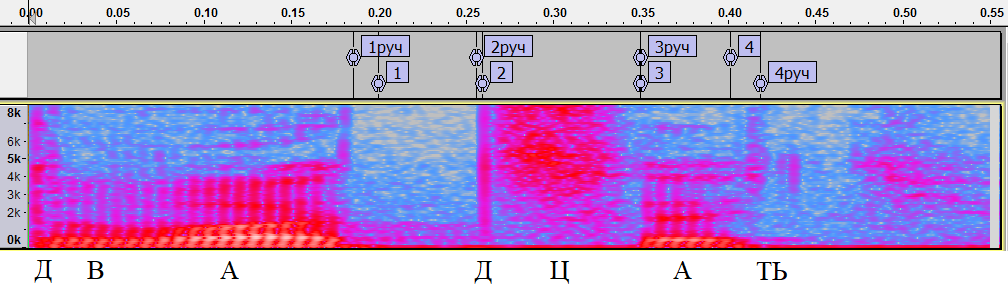
\includegraphics[width=1.0\textwidth]{word_20.png}
	\caption{Спектрограмма слова <<двадцать>>}
	\label{fig:word_20}
\end{figure}

\begin{table}[h]
	\centering
	\caption{Границы частей для разных критериев, слово <<двадцать>>}
	\label{tab:results_20}
	{\normalsize
		\begin{tabular}{| l | c | c | c | c | c | c | c | c | c | c | c |}
			\hline
			\multirow{2}{*}{Функционал} & \multicolumn{4}{c|}{Границы частей, с} & Значение \\
			\hhline{~----~} & \phantom{000} 1 \phantom{000} & \phantom{000} 2 \phantom{000} & \phantom{000} 3 \phantom{000} & \phantom{000} 4 \phantom{000} & \phantom{00}функционала\phantom{00} \\
			\hline
			$J_{1}$		& 0.20 & 0.26 & 0.35 & 0.40 & 0.67 \\
			$J_{2}$		& 0.20 & 0.26 & 0.35 & 0.39 & 0.01 \\
			$J_{3}$		& 0.20 & 0.26 & 0.35 & 0.39 & 0.15 \\
			$J_{12}$	& 0.20 & 0.26 & 0.35 & 0.40 & 0.66 \\
			$J_{123}$	& 0.20 & 0.26 & 0.35 & 0.40 & 0.51 \\
			\hline
			Вручную		& 0.18 & 0.25 & 0.35 & 0.41 & --- \\
			\hline
		\end{tabular}
	}
\end{table}

Разбиение слова <<пилотаж>> показано на рисунке \ref{fig:word_pilotage}.
В первой части слова находится звук <<п>>, во второй --- <<ило>>, после чего следует придыхание, за которым звучит <<та>> и в последней части находится звук <<ш>>.

\begin{figure}[h]
	\centering
	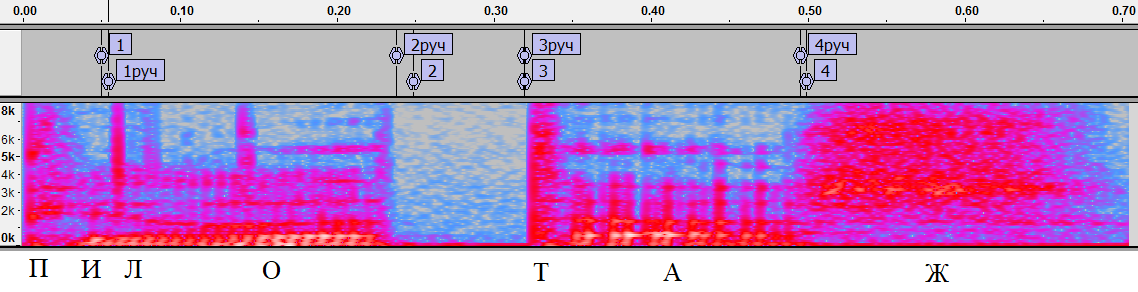
\includegraphics[width=1.0\textwidth]{word_pilotage.png}
	\caption{Спектрограмма слова <<пилотаж>>}
	\label{fig:word_pilotage}
\end{figure}

На рисунке \ref{fig:word_navigation} приведено слово <<навигация>>.
Первая часть --- это придыхание перед звуком <<н>>, далее идут части со слогами <<на>>, <<ви>> и <<га>>.
Последняя часть содержит звуки <<ция>>.

\begin{figure}[h]
	\centering
	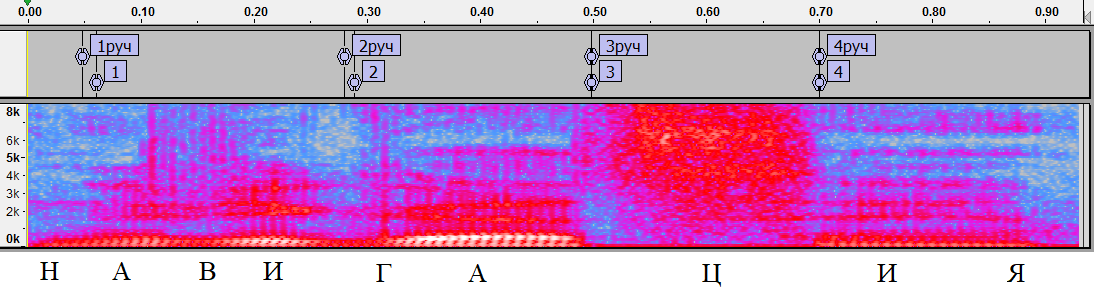
\includegraphics[width=1.0\textwidth]{word_navigation.png}
	\caption{Спектрограмма слова <<навигация>>}
	\label{fig:word_navigation}
\end{figure}

На рисунке \ref{fig:word_less} представлено слово <<меньше>>. Первая часть содержит звуки <<мень>>, затем идёт звук <<ш>> и третья часть представляет собой звук <<е>>.

\begin{figure}[h]
	\centering
	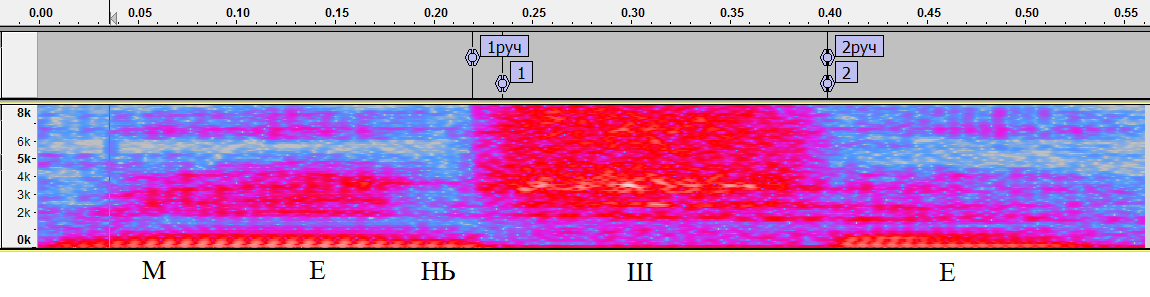
\includegraphics[width=1.0\textwidth]{word_less.png}
	\caption{Спектрограмма слова <<меньше>>}
	\label{fig:word_less}
\end{figure}

Анализ показывает достаточно хорошее совпадение границ, найденных автоматически, и эталонных границ, полученных в ручном режиме обработки.
Как правило, обнаружить различия можно во время пауз при произнесении слова.
К примеру, в слове <<двадцать>> перед <<ть>>, а в слове <тысяча>> до произнесения <<ч>>.
Проведённая обработка показывает также, что результаты, полученные при помощи различных критериев, близки между собой, особенно в тех случаях, когда однородные части содержат отдельные звуки, что соответствует допущениям, принятым при формировании критериев.
Из чего следует, что разработанные алгоритмы автоматического разделения слов на фонетически однородные части являются работоспособными.

Разработан метод автоматического разбиения слов на однородные доли по фонетическим показателям, в основе которого лежит нахождение результата с помощью многопараметрической оптимизации.
Были разработаны критерии, позволяющие воплотить принцип достижения максимального значения фонетического сходства материала в рамках одной части и значения разнородности смежных частей.
Алгоритмы, в основе которых лежит подход динамического программирования, предложены для нахождения численных результатов при решении задач с высоким быстродействием.
Адекватность принятых допущений и работоспособность данного метода были подтверждены экспериментально на примере нескольких русских слов.

По итогам выполненных экспериментов наилучшие показатели распознавания были получены при использовании первого функционала $J_1$.
К общим выводам можно отнести то, что использование простых функционалов при разбиении слов на однородные части даёт очень точное разбиение.
Сейчас получены улучшения результатов распознавания слов при использовании ручного разбиения эталона.
Использование автоматического разбиения слов также может помочь автоматизировать процесс распознавания и сократить количество ошибок.

%\newpage
%============================================================================================================================

\section{Результаты проверки работоспособности алгоритма формирования оптимального эталона на основе метода главных компонент} \label{sect3_3}

\subsection{Проверка эффективности выделения главных компонент} \label{sect3_3_1}

Проверка эффективности алгоритма выделения главных компонент на основе теории, описанной в подразделе \ref{sect2_3_1}, была выполнена следующим образом.
Анализ проводился в отдельности для каждого из трёх слов <<пилотаж>>, <<масштаб>>, <<навигация>> одного диктора.
В качестве $М$ исходных матриц \eqref{eq:2_3_1_1} были выбраны параметрические портреты всех реализаций каждого слова диктора Н-ов, то есть было составлено всего 3 различных матрицы $Х$ согласно \eqref{eq:2_3_1_2} с количеством столбцов равным 53, 44 и 53 для слов <<пилотаж>>, <<масштаб>>, <<навигация>> соответственно.

По формулам \eqref{eq:2_3_1_4} и \eqref{eq:2_3_1_5} можно вычислить первые $M'$ главных компонент, где $M'$ определяется условиями задачи. 
А оценку погрешности перехода к $M'$ главным компонентам можно рассчитать по формуле \eqref{eq:2_3_1_6}.

Сравнение, например, первой главной компоненты каждого слова с соответствующим эталоном $E$, сформированным как среднее по всем реализациям конкретного слова для выбранного диктора можно провести по формуле 

\begin{equation} \label{eq:3_3_1_1}
\epsilon_1 = \frac{||E - \widehat{k}_1 a_1 - \widehat{b}_0||}{||E||},
\end{equation}
где $||E|| = \sqrt{e_1^2 + e_2^2 + \dots + e_p^2}$ --- элементы вектора $E$ имеющего размерность $p$;

\begin{equation} \label{eq:3_3_1_2}
\widehat{k}_1 = \frac{\sum_{i=1}^p (e_i - \widehat{m}_e)(a_{1i} - \widehat{m}_{a1})}{\sum_{i=1}^p (a_{1i} - \widehat{m}_{a1})^2},	
\end{equation}

\begin{equation} \label{eq:3_3_1_3}
\widehat{b}_0 = \widehat{m}_e - \widehat{k}_1 \widehat{m}_{a1},
\end{equation}
\begin{itemize}[align=left,leftmargin=1.8em,itemindent=0pt,labelsep=0pt,labelwidth=1.8em]
	\item[где] $\widehat{m}_e = \frac{1}{p} \sum_{i=1}^p e_i$,
	\item[] $\widehat{m}_{a1} = \frac{1}{p} \sum_{i=1}^p a_{1i}$.
\end{itemize}

Формулы \eqref{eq:3_3_1_2} и \eqref{eq:3_3_1_3} есть оценки линейной парной регрессии, вычисленные по методу наименьших квадратов.

Предлагается вычислить первые $M' = 6$ главных компонент $a_1, a_2, \dots, a_6$ и проверить их на ортогональность.
Для этого нужно сформировать матрицу размерности $p \times 6$: $A_{p \times 6} = [a_1 a_2 a_3 a_4 a_5 a_6]$.
И затем вычислить матрицу размерности $6 \times 6$:

\begin{equation} \label{eq:3_3_1_4}
A_{6 \times 6} = A_{p \times 6}^T A_{p \times 6}.
\end{equation}

Если главные компоненты ортогональны, то матрица $A_{6 \times 6}$ является диагональной, то есть её недиагональные элементы на несколько порядков меньше диагональных. 

В матрицах \eqref{eq:3_3_1_5}--\eqref{eq:3_3_1_7} приведены результаты, подсчитанные по формуле \eqref{eq:3_3_1_4}.

\begin{equation} \label{eq:3_3_1_5}
A_{6 \times 6}^{\text{пилотаж}} =
\begin{bmatrix}
34765.9	& 0.0	& 0.0	& 0.0	& 0.0	& 0.0	\\
0.0		& 318.1	& 0.0	& 0.0	& 0.0	& 0.0	\\
0.0		& 0.0	& 84.5	& 0.0	& 0.0	& 0.0	\\
0.0		& 0.0	& 0.0	& 59.1	& 0.0	& 0.0	\\
0.0		& 0.0	& 0.0	& 0.0	& 41.7	& 0.0	\\
0.0		& 0.0	& 0.0	& 0.0	& 0.0	& 26.5	\\
\end{bmatrix},
\end{equation}

\begin{equation} \label{eq:3_3_1_6}
A_{6 \times 6}^{\text{масштаб}} =
\begin{bmatrix}
29516.8	& 0.0	& 0.0	& 0.0	& 0.0	& 0.0	\\
0.0		& 176.0	& 0.0	& 0.0	& 0.0	& 0.0	\\
0.0		& 0.0	& 82.3	& 0.0	& 0.0	& 0.0	\\
0.0		& 0.0	& 0.0	& 78.4	& 0.0	& 0.0	\\
0.0		& 0.0	& 0.0	& 0.0	& 63.1	& 0.0	\\
0.0		& 0.0	& 0.0	& 0.0	& 0.0	& 35.7	\\
\end{bmatrix},
\end{equation}

\begin{equation} \label{eq:3_3_1_7}
A_{6 \times 6}^{\text{навигация}} =
\begin{bmatrix}
32611.7	& 0.0	& 0.0	& 0.0	& 0.0	& 0.0	\\
0.0		& 257.3	& 0.0	& 0.0	& 0.0	& 0.0	\\
0.0		& 0.0	& 72.9	& 0.0	& 0.0	& 0.0	\\
0.0		& 0.0	& 0.0	& 56.5	& 0.0	& 0.0	\\
0.0		& 0.0	& 0.0	& 0.0	& 42.6	& 0.0	\\
0.0		& 0.0	& 0.0	& 0.0	& 0.0	& 32.7	\\
\end{bmatrix}.
\end{equation}

Внедиагональные элементы являются величинами порядка 10$^{-12}$--10$^{-14}$, что близко к ошибкам округления при скалярном перемножении векторов главных компонент.
Так как они весьма близки к нулю, можно сделать вывод, что экспериментальные данные подтверждают ортогональность главных компонент.
Также следует отметить, что скалярный квадрат первой главной компоненты на два порядка выше, чем у остальных пяти главных компонент, что свидетельствует о её весомости.

Далее разложим эталон по главным компонентам методом множественной линейной регрессии, то есть найдём оценки параметров $b_0, k_1, k_2, k_3, k_4, k_5, k_6$ соответствующие модели \eqref{eq:2_3_1_4}.	
Для этого сформируем вектор 

\begin{equation}
b = \begin{bmatrix} b_0 \\ k_1 \\ k_2 \\ k_3 \\ k_4 \\ k_5 \\ k_6 \end{bmatrix} \text{ , }
A_0 = \begin{bmatrix} 1 \\ 1 \\ \vdots \\ 1 \end{bmatrix} \text{ --- единичный вектор размерности } p
\end{equation}
и матрицу размерности $p \times 7$

\begin{equation}
A_{p \times 7} = [A_0 | A_{p \times 6}] = [A_0 A_1 A_2 A_3 A_4 A_5 A_6].
\end{equation}

Тогда все 7 оценок вектора коэффициентов разложения можно найти по формуле

\begin{equation} \label{eq:3_3_1_8}
\widehat{b} = (A_{p \times 7}^T A_{p \times 7})^{-1} A_{p \times 7}^T E.
\end{equation}

В таблицах \ref{tab:regressionCoefficientsPilotage}--\ref{tab:regressionCoefficientsNavigation} представлены коэффициенты разложения эталонов, полученных как среднее по всем реализациям каждого слова, по главным компонентам и константе.
Результаты, подсчитанные по формуле \eqref{eq:3_3_1_8}, приведены для всех трёх слов.

\begin{table}[h]
	\centering
	\caption{Коэффициенты разложения эталона по главным компонентам для слова <<пилотаж>>}
	\label{tab:regressionCoefficientsPilotage}
	\begin{tabular}{| l | c | c | c | c | c | c | c |}
		\hline
		\multicolumn{1}{|c|}{---} & \multicolumn{7}{c|}{Коэффициенты при главных компонентах} \\
		\hline
		Число гл. компонент & $\widehat{b}_0$ & $\widehat{b}_1$ & $\widehat{b}_2$ & $\widehat{b}_3$ & $\widehat{b}_4$ & $\widehat{b}_5$ & $\widehat{b}_6$ \\
		\hline
		1 гл. компонента & -0.0055 & 0.1369 & \multicolumn{1}{c|}{---} & \multicolumn{1}{c|}{---} & \multicolumn{1}{c|}{---} & \multicolumn{1}{c|}{---} & \multicolumn{1}{c|}{---} \\
		2 гл. компоненты &  0.0011 & 0.1372 & 0.0055 & \multicolumn{1}{c|}{---} & \multicolumn{1}{c|}{---} & \multicolumn{1}{c|}{---} & \multicolumn{1}{c|}{---} \\
		3 гл. компоненты &  0.0012 & 0.1372 & 0.0055 & -0.0015 & \multicolumn{1}{c|}{---} & \multicolumn{1}{c|}{---} & \multicolumn{1}{c|}{---} \\
		4 гл. компоненты &  0.0012 & 0.1372 & 0.0055 & -0.0015 & 0.0002 & \multicolumn{1}{c|}{---} & \multicolumn{1}{c|}{---} \\
		5 гл. компонент  &  0.0013 & 0.1372 & 0.0055 & -0.0015 & 0.0002 & 0.0002 & \multicolumn{1}{c|}{---} \\
		6 гл. компонент  &  0.0015 & 0.1372 & 0.0055 & -0.0015 & 0.0002 & 0.0002 & -0.0006 \\
		\hline
	\end{tabular}
\end{table}

\begin{table}[h]
	\centering
	\caption{Коэффициенты разложения эталона по главным компонентам для слова <<масштаб>>}
	\label{tab:regressionCoefficientsScale}
	\begin{tabular}{| l | c | c | c | c | c | c | c |}
		\hline
		\multicolumn{1}{|c|}{---} & \multicolumn{7}{c|}{Коэффициенты при главных компонентах} \\
		\hline
		Число гл. компонент & $\widehat{b}_0$ & $\widehat{b}_1$ & $\widehat{b}_2$ & $\widehat{b}_3$ & $\widehat{b}_4$ & $\widehat{b}_5$ & $\widehat{b}_6$ \\
		\hline
		1 гл. компонента & -0.0015 & 0.1506 & \multicolumn{1}{c|}{---} & \multicolumn{1}{c|}{---} & \multicolumn{1}{c|}{---} & \multicolumn{1}{c|}{---} & \multicolumn{1}{c|}{---} \\
		2 гл. компоненты & -0.0003 & 0.1507 & 0.0011 & \multicolumn{1}{c|}{---} & \multicolumn{1}{c|}{---} & \multicolumn{1}{c|}{---} & \multicolumn{1}{c|}{---} \\
		3 гл. компоненты &  0.0016 & 0.1507 & 0.0013 & 0.0019 & \multicolumn{1}{c|}{---} & \multicolumn{1}{c|}{---} & \multicolumn{1}{c|}{---} \\
		4 гл. компоненты &  0.0019 & 0.1507 & 0.0013 & 0.0020 & -0.0013 & \multicolumn{1}{c|}{---} & \multicolumn{1}{c|}{---} \\
		5 гл. компонент  &  0.0020 & 0.1507 & 0.0013 & 0.0020 & -0.0013 & 0.0010 & \multicolumn{1}{c|}{---} \\
		6 гл. компонент  &  0.0003 & 0.1507 & 0.0012 & 0.0017 & -0.0013 & 0.0010 & -0.0033 \\
		\hline
	\end{tabular}
\end{table}

\begin{table}[h]
	\centering
	\caption{Коэффициенты разложения эталона по главным компонентам для слова <<навигация>>}
	\label{tab:regressionCoefficientsNavigation}
	\begin{tabular}{| l | c | c | c | c | c | c | c |}
		\hline
		\multicolumn{1}{|c|}{---} & \multicolumn{7}{c|}{Коэффициенты при главных компонентах} \\
		\hline
		Число гл. компонент & $\widehat{b}_0$ & $\widehat{b}_1$ & $\widehat{b}_2$ & $\widehat{b}_3$ & $\widehat{b}_4$ & $\widehat{b}_5$ & $\widehat{b}_6$ \\
		\hline
		1 гл. компонента & 0.0021 & 0.1373 & \multicolumn{1}{c|}{---} & \multicolumn{1}{c|}{---} & \multicolumn{1}{c|}{---} & \multicolumn{1}{c|}{---} & \multicolumn{1}{c|}{---} \\
		2 гл. компоненты & 0.0022 & 0.1373 & 0.0003 & \multicolumn{1}{c|}{---} & \multicolumn{1}{c|}{---} & \multicolumn{1}{c|}{---} & \multicolumn{1}{c|}{---} \\
		3 гл. компоненты & 0.0021 & 0.1373 & 0.0003 & 0.0010 & \multicolumn{1}{c|}{---} & \multicolumn{1}{c|}{---} & \multicolumn{1}{c|}{---} \\
		4 гл. компоненты & 0.0023 & 0.1373 & 0.0003 & 0.0010 & 0.0013 & \multicolumn{1}{c|}{---} & \multicolumn{1}{c|}{---} \\
		5 гл. компонент  & 0.0025 & 0.1373 & 0.0003 & 0.0010 & 0.0013 & 0.0028 & \multicolumn{1}{c|}{---} \\
		6 гл. компонент  & 0.0014 & 0.1373 & 0.0003 & 0.0010 & 0.0012 & 0.0028 & -0.0016 \\
		\hline
	\end{tabular}
\end{table}

Количество главных компонент, участвующих в разложении, последовательно увеличивается от 1 до 6.
Опять же можно видеть, что наиболее значимым коэффициентом регрессии является коэффициент при первой главной компоненте.
При увеличении количества компонент изменение коэффициентов незначительное. 

Формула для нахождения рассогласования с эталоном в данном случае будет иметь вид:

\begin{equation} \label{eq:3_3_1_9}
\epsilon_6 = \frac{||E - \widehat{b}_0 - \widehat{k}_1 a_1 - \widehat{k}_2 a_2 - \widehat{k}_3 a_3 - \widehat{k}_4 a_4 - \widehat{k}_5 a_5 - \widehat{k}_6 a_6||}{||E||}.
\end{equation}

С практической точки зрения интересно посмотреть рассогласование разложения эталона, а также информационный критерий, вычисленный по формуле \eqref{eq:2_3_1_6}, последовательно увеличивая число главных компонент с 1 до 6.

Результаты вычислений по формуле \eqref{eq:2_3_1_6} для трёх слов представлены в таблице \ref{tab:informationMeasureDependence}.
Первая строка данной таблицы содержит меру информативности при использовании только одной главной компоненты.
Вторая строка показывает меру информативности, когда используются две первые главные компоненты, третья строка --- три первые главные компоненты и так далее.

\begin{table}[h]
	\centering
	\caption{Мера информативности при переходе системы к разному числу главных компонент (от 1 до 6)}
	\label{tab:informationMeasureDependence}
	\begin{tabular}{|l | c | c | c |}
		\hline
		\multicolumn{1}{|c|}{---} & \multicolumn{3}{c|}{$I_p$, мера информативности} \\
		\hline
		Число гл. компонент\phantom{000} & \phantom{000}пилотаж\phantom{000} & \phantom{000}масштаб\phantom{000} & \phantom{000}навигация\phantom{000} \\
		\hline
		1 гл. компонента	& 0.980	& 0.980	& 0.979	\\
		2 гл. компоненты	& 0.989	& 0.986	& 0.987	\\
		3 гл. компоненты	& 0.991	& 0.989	& 0.989	\\
		4 гл. компоненты	& 0.993	& 0.991	& 0.990	\\
		5 гл. компонент		& 0.994	& 0.993	& 0.992	\\
		6 гл. компонент		& 0.995	& 0.995	& 0.993	\\
		\hline
	\end{tabular}
\end{table}

Из этих результатов можно сделать вывод, что первая главная компонента несёт в себе порядка 98~\% имеющейся информации, а первые три главных компоненты 99~\%.
С дальнейшим увеличением числа главных компонент доля информации, содержащаяся в компонентах, увеличивается и при 6 главных компонентах достигает 99.5~\%.

В таблице \ref{tab:mismatchMeasure} представлена мера рассогласования эталона и полученного разложения на главные компоненты по формулам аналогичным формулам \eqref{eq:3_3_1_1} и \eqref{eq:3_3_1_9}.
Здесь, как и в предыдущих таблицах, количество главных компонент, участвующих в разложении, последовательно увеличивается от 1 до 6.
В результате перехода от разложения по 1 главной компоненте до 6 главных компонент относительное уменьшение меры рассогласования составляет порядка 50--80~\%.

\begin{table}[h]
	\centering
	\caption{Мера рассогласования эталона и разложения для 3 слов}
	\label{tab:mismatchMeasure}
	\begin{tabular}{|l | c | c | c | c | c | c |}
		\hline
		\multicolumn{1}{|c|}{---} & \multicolumn{6}{c|}{Мера рассогласования} \\
		\hline
		Слово \phantom{0000000} & \phantom{000}$\epsilon_1$\phantom{000} & \phantom{000}$\epsilon_2$\phantom{000} & \phantom{000}$\epsilon_3$\phantom{000} & \phantom{000}$\epsilon_4$\phantom{000} & \phantom{000}$\epsilon_5$\phantom{000} & \phantom{000}$\epsilon_6$\phantom{000} \\
		\hline
		пилотаж		& 0.0038	& 0.0008	& 0.0006	& 0.0006	& 0.0005	& 0.0005	\\
		масштаб		& 0.0013	& 0.0011	& 0.0010	& 0.0009	& 0.0008	& 0.0003	\\
		навигация	& 0.0011	& 0.0011	& 0.0010	& 0.0009	& 0.0006	& 0.0005	\\
		\hline
	\end{tabular}
\end{table}

Из данного подраздела можно сделать вывод, что использование 6 главных компонент является целесообразным, так они содержат около 99.5~\% информации о параметрическом портрете.

%\newpage
%============================================================================================================================

\subsection{Проверка работоспособности алгоритма на основе метода главных компонент} \label{sect3_3_2}

В данном подразделе приведена проверка работоспособности алгоритма на основе метода главных компонент, описанного в подразделе \ref{sect2_3_2}.
В ходе оптимизации методом покоординатного спуска, вычисление усреднённого значения нижней границы Z-коэффициента корреляции проводится с использованием обучающей выборки --- реализаций слов диктора Н-ов с шумом в наушниках 80 дБ, в то время как исходное разложение на главные компоненты было получено по записям того же диктора без шума.
Более подробно исследование информативности главных компонент в зависимости от их количества будет приведено в следующем подразделе.

Для поэтапного отслеживания эффективности работы метода покоординатного спуска ниже представлены таблицы \ref{tab:deltaZNoOptimization} и \ref{tab:deltaZOptimization}, в которых указано среднее значение и стандартное отклонение для величины $\Delta Z^{low}_{i}$, определённой в формуле \eqref{eq:2_3_2_2}, а также вероятность того, что данная величина, которая подчиняется нормальному закону распределения, будет иметь значение меньше нуля.
При этом, так как при распознавании возникает две величины $\Delta Z_{ij}$, показаны значения для наименьшей из них равной $\Delta Z^{low}_{i}$, согласно методологии, описанной в подразделе \ref{sect2_3_2}.

В таблице \ref{tab:deltaZNoOptimization} указаны результаты вычислений, применённых к тестовой выборке и изначальному эталону, полученному по формуле \eqref{eq:2_3_2_4} без выполнения оптимизации.

\begin{table}[h]
	\centering
	\caption{Статистические данные для величины $\Delta Z^{low}_{i}$, полученные при вычислении коэффициента корреляции на тестовой выборке и не оптимизированном эталоне}
	\label{tab:deltaZNoOptimization}
	\begin{tabular}{| l | c | c | c |}
		\hline
		Слово \phantom{0000000} & \phantom{000} $\mu(\Delta Z^{low}_{i})$ \phantom{000} & \phantom{000} $\sigma(\Delta Z^{low}_{i})$ \phantom{000} & \phantom{000} $P(\Delta Z^{low}_{i} < 0)$ \phantom{000} \\
		\hline
		пилотаж		& 0.789	& 0.177 & 4.25E-06 \\
		масштаб		& 1.212	& 0.221 & 2.21E-08 \\
		навигация	& 0.791	& 0.250 & 7.86E-04 \\
		\hline
	\end{tabular}
\end{table}

В таблице \ref{tab:deltaZOptimization} указаны результаты, полученные на тестовой выборке и эталоне, построенном после применения 5 циклов оптимизации.
Было проведено 5 циклов оптимизации простого варианта оптимизации коэффициентов разложения в формуле \eqref{eq:2_3_2_5}, так как сработал критерий остановки - увеличение значения нижней границы $\Delta Z^{low}_{i}$ после пятого цикла по сравнению с результатами значений четвёртого цикла менее чем на 2~\%.

\begin{table}[h]
	\centering
	\caption{Статистические данные для величины $\Delta Z^{low}_{i}$, полученные при вычислении коэффициента корреляции на тестовой выборке и оптимизированном эталоне после 5 циклов}
	\label{tab:deltaZOptimization}
	\begin{tabular}{| l | c | c | c |}
		\hline
		Слово \phantom{0000000} & \phantom{000} $\mu(\Delta Z^{low}_{i})$ \phantom{000} & \phantom{000} $\sigma(\Delta Z^{low}_{i})$ \phantom{000} & \phantom{000} $P(\Delta Z^{low}_{i} < 0)$ \phantom{000} \\
		\hline
		пилотаж		& 0.917	& 0.149	& 3.89E-10 \\
		масштаб		& 1.203	& 0.178	& 6.44E-12 \\
		навигация	& 0.743	& 0.211	& 2.20E-04 \\
		\hline
	\end{tabular}
\end{table}

Из таблиц \ref{tab:deltaZNoOptimization} и \ref{tab:deltaZOptimization} видно, что на тестовой выборке алгоритм работает корректно, так как вероятность неправильного распознавания $P(\Delta Z^{low}_{i} < 0)$ уменьшается для всех трёх слов.

Распознавание для всех 12 дикторов было осуществлено для того, чтобы удостовериться в хорошем качестве распознавания оптимизированным эталоном.
Использовались все дикторы, кроме диктора Н-ов, на записях которого производилась оптимизация коэффициентов.
При этом для распознавания применялись эталоны, использованные в начале подраздела, то есть полученные на речевых данных диктора Н-ов.
Здесь для краткости будут приведены результаты распознавания только для слова <<навигация>>.
Результаты распознавания для слова <<пилотаж>> и <<масштаб>> получились аналогичными.

В таблицах \ref{tab:deltaZ12DictorsNoOptimizatioNavigation} и \ref{tab:deltaZ12DictorsOptimizatioNavigation} последовательно приведены результаты распознавания для одного из тестируемых слов при использовании изначального неоптимизированного эталона и при использовании оптимизированного эталона.

\begin{table}[h]
	\centering
	\caption{Статистические данные для величины $\Delta Z$, полученные при вычислении коэффициента корреляции для 12 дикторов и не оптимизированном эталоне для слова <<навигация>>}
	\label{tab:deltaZ12DictorsNoOptimizatioNavigation}
	\begin{tabular}{| l | c | c | c |}
		\hline
		Номер диктора & \phantom{000} $\mu(\Delta Z^{low}_{i})$ \phantom{000} & \phantom{000} $\sigma(\Delta Z^{low}_{i})$ \phantom{000} & \phantom{000} $P(\Delta Z^{low}_{i} < 0)$ \phantom{000} \\
		\hline
		1	& 0.880	& 0.209	& 1.23E-05 \\
		2	& 0.878	& 0.256	& 3.02E-04 \\
		3	& 0.958	& 0.127	& 2.47E-14 \\
		4	& 0.870	& 0.094	& 1.01E-20 \\
		5	& 0.624	& 0.231	& 3.48E-03 \\
		6	& 0.778	& 0.209	& 9.88E-05 \\
		7	& 0.693	& 0.118	& 2.42E-09 \\
		8	& 0.522	& 0.163	& 6.95E-04 \\
		9	& 0.748	& 0.163	& 2.15E-06 \\
		10	& 0.857	& 0.129	& 1.36E-11 \\
		11	& 0.523	& 0.115	& 2.57E-06 \\
		12	& 0.841	& 0.163	& 1.24E-07 \\
		\hline
	\end{tabular}
\end{table}

\begin{table}[h]
	\centering
	\caption{Статистические данные для величины $\Delta Z$, полученные при вычислении коэффициента корреляции для 12 дикторов и оптимизированном эталоне для слова <<навигация>> }
	\label{tab:deltaZ12DictorsOptimizatioNavigation}
	\begin{tabular}{| l | c | c | c |}
		\hline
		Номер диктора & \phantom{000} $\mu(\Delta Z^{low}_{i})$ \phantom{000} & \phantom{000} $\sigma(\Delta Z^{low}_{i})$ \phantom{000} & \phantom{000} $P(\Delta Z^{low}_{i} < 0)$ \phantom{000} \\
		\hline
		1	& 0.817	& 0.196	& 1.51E-05 \\
		2	& 0.792	& 0.238	& 4.36E-04 \\
		3	& 0.768	& 0.114	& 7.03E-12 \\
		4	& 0.683	& 0.071	& 2.11E-22 \\
		5	& 0.562	& 0.225	& 6.25E-03 \\
		6	& 0.705	& 0.230	& 1.06E-03 \\
		7	& 0.739	& 0.110	& 9.43E-12 \\
		8	& 0.598	& 0.144	& 1.54E-05 \\
		9	& 0.646	& 0.146	& 5.01E-06 \\
		10	& 0.676	& 0.108	& 2.17E-10 \\
		11	& 0.443	& 0.116	& 6.45E-05 \\
		12	& 0.815	& 0.168	& 6.12E-07 \\
		\hline
	\end{tabular}
\end{table}

Представленные таблицы показывают, что при использовании оптимизированного эталона не всегда удаётся добиться улучшения распознавания слов дикторов, не входивших в обучающую выборку.
Для слова <<навигация>>, можно заметить, что ухудшение в значении вероятности неправильного распознавания произошло для 3, 6, 10 и 11 дикторов, для остальных дикторов было показано улучшение качества распознавания.

С целью проверить качественные показатели полученного эталона, кроме всего прочего, были идентифицированы реализации слов, не использовавшиеся для создания эталона и произносившиеся при проведении эксперимента с обратной связью.
То есть, в комнате через колонки подавался шум самолёта Boeing с уровнем громкости 80 дБ, а диктору, который зачитывал слова в наушники, подавался его же голос.
В таблице \ref{tab:errorsPercentageInitialOptimized} выведен процент ошибок распознавания для изначального эталона (1) и улучшенного эталона (2) соответственно для всех трёх слов.
Опять же можно увидеть, что улучшение распознавания наблюдается не для всех дикторов, но суммарное количество ошибок стало меньше.

\begin{table}[h]
	\centering
	\caption{Процент ошибок распознавания для всех трёх слов при использовании изначального (1) и оптимизированного (2) эталонов}
	\label{tab:errorsPercentageInitialOptimized}
	\begin{tabular}{| l | c | c | c | c | c | c |}
		\hline
		\multicolumn{1}{|c|}{---} & \multicolumn{6}{c|}{Процент ошибок} \\
		\hline
		\multicolumn{1}{|c|}{Номер} & \multicolumn{2}{c|}{пилотаж} & \multicolumn{2}{c|}{масштаб} & \multicolumn{2}{c|}{навигация} \\
		\hhline{~------}
		\multicolumn{1}{|c|}{\phantom{00} диктора \phantom{00}}& \phantom{00} (1) \phantom{00} & \phantom{00} (2) \phantom{00} & \phantom{00} (1) \phantom{00} & \phantom{00} (2) \phantom{00} & \phantom{00} (1) \phantom{00} & \phantom{00} (2) \phantom{00} \\
		\hline
		1		& 0	& 2	& 9	 & 18 & 9  & 6	\\
		2		& 0	& 0	& 95 & 95 & 92 & 81	\\
		3		& 0	& 2	& 68 & 66 & 6  & 8	\\
		4		& 0	& 0	& 36 & 41 & 2  & 6	\\
		5		& 0	& 0	& 0	 & 0  & 0  & 0	\\
		6		& 0	& 0	& 98 & 70 & 98 & 64	\\
		7		& 0	& 0	& 30 & 9  & 2  & 2	\\
		8		& 0	& 0	& 0	 & 0  & 4  & 4	\\
		9		& 0	& 0	& 2	 & 2  & 0  & 0	\\
		10		& 0	& 0	& 95 & 89 & 94 & 95	\\
		11		& 4	& 2	& 23 & 25 & 6  & 34	\\
		12		& 0	& 0	& 2	 & 2  & 0  & 0	\\
		\hline
		Среднее	& 0	& 0	& 38 & 35 & 26 & 24 \\
		\hline
	\end{tabular}
\end{table}

По результатам экспериментов в данном подразделе можно заметить, что оптимизация эталона в среднем помогает увеличить нижнюю границу дельты коэффициента корреляции и снизить количество ошибок распознавания.
При этом стоит отметить, что, несмотря на общее снижение количества ошибок, для определённых дикторов процент ошибок может увеличиваться.

\clearpage

%\newpage
%============================================================================================================================

\subsection{Распознавание с помощью алгоритма на основе метода главных компонент} \label{sect3_3_3}

В данном подразделе выполняется тестирование распознавания с помощью метода главных компонент, описанного в подразделе \ref{sect2_3_2}.
В качестве тестовых данных для распознавания использовались три слова: <<пилотаж>>, <<навигация>> и <<масштаб>>.
Они произнесены 4 дикторами в условиях с шумом в наушниках и 10 в условиях без шума \cite{korsun2014algo, korsun2012method, schmidt2000speech}.
По 10 различным дикторам в условиях без шума находятся 10 наборов эталонов для всех слов.
Они составляются путём обычного усреднения записей, наиболее близких по длине к среднему значению длины записи соответствующего слова.
Далее из этих усреднённых эталонов находятся 6 главных компонент, а потом проводится регрессия усреднённого эталона на константу и полученные 6 главных компонент.
В результате этого получаются коэффициенты при главных компонентах.
Далее с использованием обучающей выборки, состоящей из записей диктора Н-ов с шумом в наушниках 80 дБ, была произведена оптимизация коэффициентов при главных компонентах.

Распознавание всех команд второго набора, надиктованного 4 дикторами со значениями шума в наушниках 80 дБ и 90 дБ было проведено в качестве тестирования качества оптимизированного эталона.
Результаты представлены в таблицах \ref{tab:subsect3_3_3_tab1} и \ref{tab:subsect3_3_3_tab2}.

\begin{table}[h]
	\centering
	\caption{Результаты распознавания записей с шумом в наушниках 80 дБ на обычном (1) и оптимизированном (2) эталонах}
	\label{tab:subsect3_3_3_tab1}
	\begin{tabular}{| c | c | c | c |}
		\hline
		\phantom{000} Диктор \phantom{000} & \phantom{000000} Слово \phantom{000000} & \phantom{000} Ошибки 1 \phantom{000} & \phantom{000} Ошибки 2 \phantom{000} \\
		\hline
				& пилотаж	& 6 & 0 \\
		Б-ак	& масштаб   & 0 & 0 \\
				& навигация & 0 & 8 \\
		\hline
				& пилотаж	& 3 & 0 \\
		Г-ов	& масштаб   & 0 & 0 \\
				& навигация & 0 & 0 \\
		\hline
				& пилотаж	& 8 & 0 \\
		Н-ов	& масштаб   & 0 & 0 \\
				& навигация & 0 & 0 \\
		\hline
				& пилотаж	& 9 & 0 \\
		Ф-ев	& масштаб   & 0 & 0 \\
				& навигация & 0 & 0 \\
		\hline
		\multicolumn{2}{|c|}{Суммарные результаты} & \multicolumn{2}{c|}{\textbf{26} $\quad\longrightarrow\quad$ \textbf{8}} \\
		\hline
	\end{tabular}
\end{table}

\begin{table}[h]
	\centering
	\caption{Результаты распознавания записей с шумом в наушниках 90 дБ на обычном (1) и оптимизированном (2) эталонах}
	\label{tab:subsect3_3_3_tab2}
	\begin{tabular}{| c | c | c | c |}
		\hline
		\phantom{000} Диктор \phantom{000} & \phantom{000000} Слово \phantom{000000} & \phantom{000} Ошибки 1 \phantom{000} & \phantom{000} Ошибки 2 \phantom{000} \\
		\hline
				& пилотаж	& 7 & 0 \\
		Б-ак	& масштаб   & 0 & 0 \\
				& навигация & 0 & 1 \\
		\hline
				& пилотаж	& 3 & 0 \\
		Г-ов	& масштаб   & 0 & 0 \\
				& навигация & 0 & 2 \\
		\hline
				& пилотаж	& 12 & 0 \\
		Н-ов	& масштаб   & 0  & 0 \\
				& навигация & 0  & 0 \\
		\hline
				& пилотаж	& 4 & 0 \\
		Ф-ев	& масштаб   & 0 & 0 \\
				& навигация & 8 & 4 \\
		\hline
		\multicolumn{2}{|c|}{Суммарные результаты} & \multicolumn{2}{c|}{\textbf{34} $\quad\longrightarrow\quad$ \textbf{7}} \\
		\hline
	\end{tabular}
\end{table}

Результаты эксперимента показывают повышение качества распознавания алгоритма не только для записей слов диктора Н-ов, входящего в обучающую выборку, но и для всех остальных дикторов, при использовании оптимизированного эталона.
В распознавании было использовано 1200 записей.
Общее количество ошибок для 3 слов до оптимизации равнялось 60 или 5~\%, а после оптимизации уменьшилось до 15 или 1.25~\%.

Здесь и далее в работе будут приводиться точечные результаты оценки среднего процента правильных распознаваний.
Доверительные интервалы редко применяются при оценке результатов алгоритмов распознавания речи нескольким причинам \cite{karpov2012methodology}.
Во-первых, доверительные интервалы оказываются весьма широкими из-за большой вариативности голосов дикторов.
Во-вторых, обычно различные методы сравниваются на одинаковых тестовых базах данных записей, поэтому ширина доверительных интервалов не является информативной.
И, в-третьих, оценка доверительного интервала может оказаться ненадёжной при использовании записей одного или нескольких дикторов, так как нарушается условие независимости записей.

Кроме того, важно указать на положительные результаты распознавания при использовании неоптимизированного эталона, исходные коэффициенты разложения по главным компонентам которого были рассчитаны путём разложения усреднённого эталона.
Например, с самого начала имелась только 1 ошибка в слове <<навигация>>, произнесённого восьмым диктором.
Избавиться от данной ошибки удалось посредством оптимизации для записей без шума.

Кроме этого был проведён тест, в котором использовалось ограниченное количество реализаций слов, применяемых для получения оптимального эталона.
Результаты данных экспериментов приведены в таблице \ref{tab:subsect3_3_3_tab3}.

\begin{table}[h]
	\centering
	\caption{Результаты распознавания записей с шумом в наушниках для различного числа используемых реализаций слова и итераций при оптимизации для 3 слов}
	\label{tab:subsect3_3_3_tab3}
	{\small
		\begin{tabular}{ | l | l | l | c | c | c | c | c || c | c | c | c | c || c | c | c | c | c |}
			\hline
			\multicolumn{2}{|c|}{\textbf{\textsc{с шумом в}}} & Реализации & \multicolumn{5}{c||}{1} & \multicolumn{5}{c||}{3} & \multicolumn{5}{c|}{10} \\
			\cline{3-18}
			\multicolumn{2}{|c|}{\textbf{\textsc{\phantom{0}наушниках\phantom{0}}}} & Итерации & 0 & 1 & 3 & 10 & 30 & 0 & 1 & 3 & 10 & 30 & 0 & 1 & 3 & 10 & 30  \\
			\hline
			Диктор 	& Шум 	& Слово 	& \multicolumn{15}{c|}{Число ошибок}	\\
			\hline
					& 		& пилотаж 	& 0  & 0  & 0  & 0  & 0    & 0  & 0  & 0  & 0  & 0    & 0  & 0  & 0  & 0  & 0  \\
			Ф-ев	& 0 дБ	& масштаб 	& 0  & 0  & 0  & 0  & 0    & 0  & 0  & 0  & 0  & 0    & 0  & 0  & 0  & 0  & 0  \\
					& 		& навигация & 0  & 0  & 0  & 0  & 0    & 0  & 0  & 0  & 0  & 0    & 0  & 0  & 0  & 0  & 0  \\
			\hline
					& 		& пилотаж 	& 6  & 3  & 2  & 3  & 3    & 6  & 3  & 2  & 3  & 3    & 6  & 3  & 2  & 3  & 3  \\
			Ф-ев	& 80 дБ	& масштаб 	& 0  & 0  & 0  & 0  & 0    & 0  & 0  & 0  & 0  & 0    & 0  & 0  & 0  & 0  & 0  \\
					& 		& навигация & 0  & 0  & 0  & 0  & 0    & 0  & 0  & 0  & 0  & 0    & 0  & 0  & 0  & 0  & 0  \\
			\hline
					& 		& пилотаж 	& 1  & 1  & 0  & 0  & 0    & 1  & 1  & 0  & 0  & 0    & 1  & 1  & 0  & 0  & 0  \\
			Ф-ев  & 90 дБ	& масштаб 	& 0  & 0  & 0  & 0  & 0    & 0  & 0  & 0  & 0  & 0    & 0  & 0  & 0  & 0  & 0  \\
					& 		& навигация & 2  & 2  & 2  & 0  & 0    & 2  & 2  & 2  & 0  & 0    & 2  & 2  & 2  & 0  & 0  \\
			\hline
		\end{tabular}
	}
\end{table}

Также, вместо критерия остановки, описание которому дано в формуле \eqref{eq:2_3_2_5}, была исследована возможность применения заранее фиксированного количества итераций для оптимизации эталона.
В ходе эксперимента были использованы три тестовых выборки одного диктора с разными вариантами шума в наушниках.

Также был проведён аналогичный эксперимент, но с использованием записей других дикторов без шума.
Результаты этого эксперимента приведены в таблице \ref{tab:subsect3_3_3_tab4}.

\begin{table}[h]
	\centering
	\caption{Результаты распознавания записей с шумом в наушниках для различного числа используемых реализаций слова и итераций при оптимизации для 3 слов}
	\label{tab:subsect3_3_3_tab4}
	{\small
		\begin{tabular}{ | l | l | c | c | c | c | c || c | c | c | c | c || c | c | c | c | c |}
			\hline
			\multicolumn{1}{|c|}{\textbf{\textsc{без}}} & Реализации\phantom{0000} & \multicolumn{5}{c||}{1} & \multicolumn{5}{c||}{3} & \multicolumn{5}{c|}{10} \\
			\cline{2-17}
			\multicolumn{1}{|c|}{\textbf{\textsc{\phantom{00}шума\phantom{00}}}} & Итерации & 0 & 1 & 3 & 10 & 30 & 0 & 1 & 3 & 10 & 30 & 0 & 1 & 3 & 10 & 30 \\
			\hline
			Диктор 		& Слово 	& \multicolumn{15}{c|}{Число ошибок}	\\
			\hline
					& пилотаж 	& 0  & 0  & 0  & 0  & 0    & 0  & 0  & 0  & 0  & 0    & 0  & 0  & 0  & 0  & 0  \\
			К-ов	& масштаб 	& 0  & 0  & 0  & 0  & 0    & 0  & 0  & 0  & 0  & 0    & 0  & 0  & 0  & 0  & 0  \\
					& навигация & 7  & 5  & 0  & 0  & 0    & 7  & 5  & 0  & 0  & 0    & 7  & 5  & 0  & 0  & 0  \\
			\hline
					& пилотаж 	& 0  & 0  & 0  & 0  & 0    & 0  & 0  & 0  & 0  & 0    & 0  & 0  & 0  & 0  & 0  \\
			О-ин	& масштаб 	& 0  & 0  & 0  & 0  & 0    & 0  & 0  & 0  & 0  & 0    & 0  & 0  & 0  & 0  & 0  \\
					& навигация & 0  & 0  & 0  & 0  & 0    & 0  & 0  & 0  & 0  & 0    & 0  & 0  & 0  & 0  & 0  \\
			\hline
					& пилотаж 	& 0  & 0  & 0  & 0  & 0    & 0  & 0  & 0  & 0  & 0    & 0  & 0  & 0  & 0  & 0  \\
			С-ев	& масштаб 	& 6  & 5  & 0  & 0  & 1    & 6  & 5  & 1  & 0  & 0    & 6  & 5  & 1  & 0  & 0  \\
					& навигация & 0  & 0  & 1  & 1  & 1    & 0  & 0  & 1  & 1  & 1    & 0  & 0  & 1  & 1  & 1  \\
			\hline
					& пилотаж 	& 1  & 1  & 1  & 1  & 1    & 1  & 1  & 1  & 1  & 1    & 1  & 1  & 1  & 1  & 1  \\
			Ц-ин  	& масштаб 	& 0  & 0  & 0  & 0  & 0    & 0  & 0  & 0  & 0  & 0    & 0  & 0  & 0  & 0  & 0  \\
					& навигация & 0  & 0  & 0  & 0  & 0    & 0  & 0  & 0  & 0  & 0    & 0  & 0  & 0  & 0  & 0  \\
			\hline
		\end{tabular}
	}
\end{table}

В обоих случаев постановки эксперимента видно, что количество ошибок уменьшается с увеличением количеством итераций обучения, при этом никак не зависит от числа использованных записей.

Полученные в ходе эксперимента данные позволяют сделать вывод о том, что 1 реализации слова достаточно для вычисления оптимального эталона.
Для получения устойчивых результатов чаще всего достаточным значением являются 10 итераций, поскольку их увеличение не способствует повышению результатов.
Полученный вывод имеет большое значение в целях снижения временных затрат при оптимизации эталонов, поскольку количественное увеличение реализаций слов для получения релевантного эталона приводит к линейному росту временных затрат при работе алгоритма.

Полученный путём оптимизации коэффициентов при главных компонентах эталон продемонстрировал возможность распознавания большинства записей с существенно меньшим количеством ошибок.
Рассматриваемый алгоритм показал себя подходящим методом распознавания слов, уменьшающим число ошибок в данной задаче \cite{kolokolov2015compare}, как и алгоритм разделения слов на однородные части.
Редко встречаются случаи увеличения числа ошибок, что, скорее всего, обусловлено попаданием алгоритма в локальный, а не глобальный экстремум при использовании метода покоординатного спуска.
Ввиду этого есть смысл использовать более релевантный метод числовой оптимизации.
Также было замечено, что в качестве записей для эталона лучше использовать записи без шума, чем записи с шумом, несмотря на то что распознаваемые записи содержат шум.

Также был получен вывод о том, что для получения приемлемых результатов достаточно использовать только одну реализацию слова и проводить всего 10 итераций при получении оптимального эталона, что заметно сокращает время работы программы.

\clearpage

%\newpage
%============================================================================================================================

\section{Результаты экспериментов по формированию эталонов на основе полиномов Чебышёва} \label{sect3_4}

В данном подразделе описываются результаты экспериментов, связанных с аппроксимацией параметрических портретов полиномами Чебышёва, подробно описанной в подразделе \ref{sect2_4}.
Так как параметрический портрет представляет собой двухмерную матрицу, то аппроксимация может проводить как по временному измерению, так и по частотному.
Также можно проводить аппроксимацию по одному измерению, а затем по другому.
Наиболее оптимальным в плане уменьшения размера параметрического портрета оказалось одновременное сжатие и по частотным полосам, и по временным интервалам.

Эксперимент проводился на параметрических портретах 20 слов, произнесённых 9 различными дикторами.
При использовании исходных записей без сжатия было получено 10.7~\% ошибок при распознавании по <<чужому>> эталону и 1.6~\% ошибок при распознавании по <<своему>> эталону.
Данные результаты будут применяться для сравнения результатов распознавания после сжатия параметрических портретов распознаваемых записей.

В таблицах \ref{tab:chebyshevTest}--\ref{tab:chebyshevTrain} приведены проценты ошибок распознаваний в случае использования различного количества полиномов для обоих вариантов распознавания.

\begin{table}[h]
	\centering
	\caption{Процент ошибок при распознавании по <<чужому>> эталону для случая сжатия параметрического портрета заданным числом полиномов Чебышёва}
	\label{tab:chebyshevTest}
	\begin{tabular}{| l | c | c | c | c | c | c | c | c | c |}
		\hline
		Частотные & \multicolumn{9}{c|}{Временные интервалы} \\
		\hhline{~---------}
	 	полосы & \phantom{0} \textbf{8} \phantom{0} & \phantom{0}\textbf{10} \phantom{0} & \phantom{0}\textbf{12} \phantom{0} & \phantom{0}\textbf{14} \phantom{0} & \phantom{0}\textbf{16} \phantom{0} & \phantom{0}\textbf{18} \phantom{0} & \phantom{0}\textbf{20} \phantom{0} & \phantom{0}\textbf{22} \phantom{0} & \phantom{0}\textbf{24} \phantom{0} \\
		\hline
		\textbf{8}  & 15.7 & 16.0 & 16.5 & 16.7 & 16.8 & 16.9 & 17.1 & 17.1 & 17.1 \\
		\textbf{10} & 15.3 & 12.9 & 12.9 & 12.9 & 13.1 & 13.3 & 13.3 & 13.3 & 13.2 \\
		\textbf{12} & 15.3 & 12.8 & 11.8 & 11.9 & 11.9 & 12.0 & 12.1 & 12.1 & 12.1 \\
		\textbf{14} & 15.4 & 12.8 & 11.7 & 11.4 & 11.4 & 11.5 & 11.6 & 11.5 & 11.5 \\
		\textbf{16}	& 15.5 & 12.9 & 11.8 & 11.3 & 11.1 & 11.2 & 11.2 & 11.2 & 11.2 \\
		\textbf{18} & 15.5 & 12.8 & 11.8 & 11.3 & 11.1 & \textbf{10.9} & 10.9 & 10.8 & 10.9 \\
		\textbf{20} & 15.5 & 12.9 & 11.8 & 11.3 & 11.1 & 10.9 & 10.8 & 10.8 & 10.8 \\
		\textbf{22} & 15.4 & 12.8 & 11.8 & 11.3 & 11.1 & 10.9 & 10.8 & 10.8 & 10.8 \\
		\textbf{24} & 15.4 & 12.8 & 11.8 & 11.3 & 11.1 & 10.9 & 10.8 & 10.8 & 10.7 \\
		\hline
	\end{tabular}
\end{table}

\begin{table}[h]
	\centering
	\caption{Процент ошибок при распознавании по <<своему>> эталону для случая сжатия параметрического портрета заданным числом полиномов Чебышёва}
	\label{tab:chebyshevTrain}
	\begin{tabular}{| l | c | c | c | c | c | c | c | c | c |}
		\hline
		Частотные & \multicolumn{9}{c|}{Временные интервалы} \\
		\hhline{~---------}
	 	полосы & \phantom{0} \textbf{8} \phantom{0} & \phantom{0}\textbf{10} \phantom{0} & \phantom{0}\textbf{12} \phantom{0} & \phantom{0}\textbf{14} \phantom{0} & \phantom{0}\textbf{16} \phantom{0} & \phantom{0}\textbf{18} \phantom{0} & \phantom{0}\textbf{20} \phantom{0} & \phantom{0}\textbf{22} \phantom{0} & \phantom{0}\textbf{24} \phantom{0} \\
		\hline
		\textbf{8}  & 2.4 & 2.4 & 2.7 & 2.9 & 3.1 & 3.2 & 3.2 & 3.2 & 3.3 \\
		\textbf{10} & 2.3 & 2.1 & 2.1 & 2.2 & 2.3 & 2.4 & 2.5 & 2.5 & 2.5 \\
		\textbf{12} & 2.5 & 2.2 & 2.0 & 2.1 & 2.1 & 2.2 & 2.2 & 2.2 & 2.2 \\
		\textbf{14} & 2.6 & 2.3 & 2.0 & 1.9 & 2.0 & 2.1 & 2.1 & 2.1 & 2.0 \\
		\textbf{16} & 2.9 & 2.4 & 2.0 & 1.9 & 1.9 & 1.9 & 2.0 & 2.0 & 1.9 \\
		\textbf{18} & 2.9 & 2.6 & 2.1 & 2.0 & 2.0 & \textbf{1.8} & 1.9 & 1.9 & 1.9 \\
		\textbf{20} & 2.9 & 2.5 & 2.1 & 2.0 & 2.0 & 1.9 & 1.9 & 1.8 & 1.9 \\
		\textbf{22} & 2.9 & 2.5 & 2.2 & 2.0 & 1.9 & 1.9 & 1.8 & 1.8 & 1.8 \\
		\textbf{24} & 2.9 & 2.5 & 2.2 & 2.0 & 1.9 & 1.8 & 1.8 & 1.7 & 1.8 \\
		\hline
	\end{tabular}
\end{table}

Сначала проводилось сжатие по частотным полосам, количество полиномов указано в первом столбце.
Затем проводилось сжатие полученного портрета по временным интервалам и тут количество использованных полиномов указано в первой строке.
Эксперимент проводился для распознавания по <<чужому>> и по <<своему>> эталону.

По результатам видно, что для обоих случаев результаты совпадают в пределах приемлемой погрешности в 0.2 процентных пункта при использовании 18 полиномов в разложении по обоим измерениям.
Это позволяет уменьшить число элементов в параметрическом портрете более чем в 5 раз.
Полное совпадение количества ошибок достигается при очень большом числе полиномов, позволяя лишь незначительно уменьшить размеры параметрического портрета.

%\newpage
%============================================================================================================================

\section{Результаты проверки работоспособности алгоритмов формирования эталонов на основе формулы Байеса и метода комитетов} \label{sect3_5}

В данном подразделе приведена проверка результатов распознавания речевых команд при распознавании алгоритмом на основе формулы Байеса и метода комитетов, описанными в подразделе \ref{sect2_5}.
Проверка алгоритмом распознавания была проведена на речевой базе, включающей в себя 20 различных изолированных слов для 8 различных дикторов.
Все слова проговаривались по 30 раз.
В данном случае количественные показатели объёма речевой базы характеризуются значением 4800 для реализации слов по 600 реализаций на каждого диктора в отдельности.
Все эксперименты проводились при использовании дикторонезависимого варианта распознавания.
Это удалось реализовать посредством исключения из распознаваемых записей тех речевых записей, которые принадлежали дикторами, записи которых применялись при формировании эталона.
При распознавании применялась мера близости между матрицами параметрических портретов, представляющая собой усреднённое по столбцам Z-преобразование Фишера от коэффициентов корреляции.
В подразделе \ref{sect1_4_1} уже было дано описание данной скалярной меры близости и был расписан алгоритм её расчёта.

Результаты экспериментов представлены ниже в таблицах \ref{tab:subsect3_2_3_tab1}--\ref{tab:subsect3_2_3_tab4}.
Вариант распознавания представлен в столбце №1 каждой из таблиц.
Символ <<1\_1>> отображает распознавание по одному эталону, сформированному по аудиозаписи лишь одного диктора.
Обозначение <<1>> соответствует распознаванию с точностью до единственного слова, а обозначения <<2>> и <<3>> --- распознаванию с точностью до группы из 2 или 3 слов.
В данном случае ошибкой распознавания признается результат, при котором в группе из 2 или 3 слов с наиболее высокими показателями нельзя обнаружить истинное слово.
В последующих столбцах для всех исследуемых дикторов даны доли неправильных распознаваний в процентах от общего числа реализаций по этому диктору.
Другими словами, значение 1.00~\% соответствует 6 ошибкам.

Результаты для алгоритма на основе формулы Байеса приведены в таблице \ref{tab:subsect3_2_3_tab1} для 3 дикторов и в таблице \ref{tab:subsect3_2_3_tab2} для 7 дикторов.

\begin{table}[h]
	\centering
	\caption{Процент ошибок при распознавании алгоритмом на основе формулы Байеса по 3 эталонам}
	\label{tab:subsect3_2_3_tab1}
	\begin{tabular}{| l | c | c | c | c | c | c | c | c | c |}
		\hline
		Вариант & \multicolumn{8}{c|}{Порядковый номер диктора} & Среднее \\
		\hhline{~--------}
		распознавания & \phantom{0} 1 \phantom{0} & \phantom{0} 2 \phantom{0} & \phantom{0} 3 \phantom{0} & \phantom{0} 4 \phantom{0} & \phantom{0} 5 \phantom{0} & \phantom{0} 6 \phantom{0} & \phantom{0} 7 \phantom{0} & \phantom{0} 8 \phantom{0} & значение \\
		\hline
		$1\_1$	& 5.33 & 9.33 & 14.5 & 8.00 & 5.00 & 11.5 & 7.00 & 6.67 & 8.42 \\
		$1$		& 7.67 & 12.5 & 14.3 & 14.7 & 11.3 & 10.3 & 5.50 & 11.0 & 10.91 \\
		$2$		& 5.83 & 9.83 & 7.33 & 12.8 & 7.17 & 5.17 & 3.33 & 8.17 & 7.45 \\
		$3$		& 5.50 & 8.83 & 6.33 & 12.2 & 5.83 & 4.00 & 3.17 & 7.33 & 6.65 \\
		\hline
	\end{tabular}
\end{table}

\begin{table}[h]
	\centering
	\caption{Процент ошибок при распознавании алгоритмом на основе формулы Байеса по 7 эталонам}
	\label{tab:subsect3_2_3_tab2}
	\begin{tabular}{| l | c | c | c | c | c | c | c | c | c |}
		\hline
		Вариант & \multicolumn{8}{c|}{Порядковый номер диктора} & Среднее \\
		\hhline{~--------}
		распознавания & \phantom{0} 1 \phantom{0} & \phantom{0} 2 \phantom{0} & \phantom{0} 3 \phantom{0} & \phantom{0} 4 \phantom{0} & \phantom{0} 5 \phantom{0} & \phantom{0} 6 \phantom{0} & \phantom{0} 7 \phantom{0} & \phantom{0} 8 \phantom{0} & значение \\
		\hline
		$1\_1$	& 5.33 & 9.33 & 14.5 & 8.00 & 5.00 & 11.5 & 7.00 & 6.67 & 8.42 \\
		$1$		& 4.83 & 7.33 & 7.33 & 4.83 & 6.50 & 6.33 & 4.67 & 3.17 & 5.62 \\
		$2$		& 2.67 & 4.83 & 3.83 & 2.17 & 2.50 & 2.67 & 2.17 & 0.83 & 2.71 \\
		$3$		& 2.50 & 3.50 & 3.00 & 1.83 & 2.17 & 2.17 & 2.00 & 0.67 & 2.23 \\	
		\hline
	\end{tabular}
\end{table}

Аналогичные результаты для алгоритма на основе метода комитетов приведены в таблице \ref{tab:subsect3_2_3_tab3} для 3 дикторов и в таблице \ref{tab:subsect3_2_3_tab4} для 7 дикторов.

\begin{table}[h]
	\centering
	\caption{Процент ошибок при распознавании алгоритмом на основе метода комитетов по 3 эталонам}
	\label{tab:subsect3_2_3_tab3}
	\begin{tabular}{| l | c | c | c | c | c | c | c | c | c |}
		\hline
		Вариант & \multicolumn{8}{c|}{Порядковый номер диктора} & Среднее \\
		\hhline{~--------}
		распознавания & \phantom{0} 1 \phantom{0} & \phantom{0} 2 \phantom{0} & \phantom{0} 3 \phantom{0} & \phantom{0} 4 \phantom{0} & \phantom{0} 5 \phantom{0} & \phantom{0} 6 \phantom{0} & \phantom{0} 7 \phantom{0} & \phantom{0} 8 \phantom{0} & значение \\
		\hline
		$1\_1$			& 5.33 & 9.33 & 14.5 & 8.00 & 5.00 & 11.5 & 7.00 & 6.67 & 8.42 \\
		$1$				& 4.17 & 8.67 & 12.5 & 10.3 & 9.67 & 10.2 & 5.67 & 7.17 & 8.54 \\
		$2$				& 1.00 & 5.17 & 4.67 & 5.00 & 5.00 & 4.00 & 1.50 & 4.83 & 3.90 \\
		$3$				& 0.50 & 3.00 & 1.50 & 1.83 & 2.83 & 2.33 & 0.83 & 1.33 & 1.77 \\
		с подстройкой	& 3.20 & 6.70 & 6.30 & 7.70 & 6.30 & 5.30 & 3.30 & 5.20 & 5.50 \\
		\hline
	\end{tabular}
\end{table}

\begin{table}[h]
	\centering
	\caption{Процент ошибок при распознавании алгоритмом на основе метода комитетов по 7 эталонам}
	\label{tab:subsect3_2_3_tab4}
	\begin{tabular}{| l | c | c | c | c | c | c | c | c | c |}
		\hline
		Вариант & \multicolumn{8}{c|}{Порядковый номер диктора} & Среднее \\
		\hhline{~--------}
		распознавания & \phantom{0} 1 \phantom{0} & \phantom{0} 2 \phantom{0} & \phantom{0} 3 \phantom{0} & \phantom{0} 4 \phantom{0} & \phantom{0} 5 \phantom{0} & \phantom{0} 6 \phantom{0} & \phantom{0} 7 \phantom{0} & \phantom{0} 8 \phantom{0} & значение \\
		\hline
		$1\_1$			& 5.33 & 9.33 & 14.5 & 8.00 & 5.00 & 11.5 & 7.00 & 6.67 & 8.42 \\
		$1$				& 4.50 & 7.33 & 7.17 & 4.83 & 4.50 & 6.67 & 4.83 & 2.83 & 5.33 \\
		$2$				& 0.67 & 3.33 & 2.83 & 1.33 & 1.67 & 2.67 & 1.00 & 1.33 & 1.85 \\
		$3$				& 0.50 & 2.50 & 1.00 & 0.50 & 1.33 & 1.67 & 0.50 & 0.50 & 1.06 \\
		с подстройкой	& 1.80 & 4.50 & 4.30 & 3.20 & 1.90 & 4.80 & 2.30 & 2.20 & 3.13 \\
		\hline
	\end{tabular}
\end{table}

Из таблиц \ref{tab:subsect3_2_3_tab1} и \ref{tab:subsect3_2_3_tab3} видно, что использование 3 эталонов почти не улучшает точность по сравнению с одним (варианты <<1\_1>> и <<1>>).
Заметное улучшение в 1.5--2 раза получаем только для 7 эталонов (таблицы \ref{tab:subsect3_2_3_tab2} и \ref{tab:subsect3_2_3_tab4}, варианты <<1\_1>> и <<1>>).
При переходе к группам из 2 и 3 слов можно достичь наилучшего эффекта.
Так, для 7 эталонов по варианту <<3>> получаем в алгоритме на основе формулы Байеса долю ошибок 0.67--3.5~\% (таблица \ref{tab:subsect3_2_3_tab2}), а в алгоритме на основе метода комитетов 0.5--2.5~\% (таблица \ref{tab:subsect3_2_3_tab4}).

Следует отметить, что возможность локализации распознаваемого слова с точностью до малой группы из 2--3 слов имеет практический смысл.
Данная процедура используется в целях значительного сокращения временных затрат на распознавания команд.
Это возможно благодаря переходу к процедуре распознавания иерархическим методом, который реализуется следующим способом: в первую очередь быстродействующие алгоритмы выделяют малую группу, после чего более затратными по времени алгоритмами проводится поиск в данной группе.
К примеру, методом сравнения с эталонами <<чужих>> слов \cite{korsun2017recognition} или посредством подстройки по длительности.
В результате чего удаётся значительно уменьшить процент ошибок при распознавании.
Данный подход более подробно описан в подразделе \ref{sect2_5_6}.
Подстройка распознаваемых слов по показателю длительности использовалась только при проведении экспериментов для алгоритмов, основанных на методе комитетов, в целях экономии времени \cite{rabiner1993fundamentals, korsun2017recognition, korsun2016automatic}

Результаты распознавания, полученные с применением подстройки по времени, представлены в строках <<с подстройкой>> таблиц \ref{tab:subsect3_2_3_tab3}--\ref{tab:subsect3_2_3_tab4}.
В использованной конфигурации подстройки использовались результаты распознавания с точностью до 2 слов, так как предварительный анализ показал, что использование большего число слов не улучшает качество распознавания, при том, что значительно увеличивает время работы алгоритма.
Также в результате предварительного анализа было выявлено, что лучшие результаты достигаются при максимальном смещении границ частей на 2 шага, каждый из которых по длительности равен 2~\% от длины слова.
По результатам видно, что подстройка по времени позволяет уменьшить процент ошибок для распознавания по 3 эталонам с 8.54 до 5.50~\%.
Учитывая, что точность распознавания до 2 слов равнялась 3.90~\%, подстройка позволяет исправить две трети ошибок, допущенных алгоритмом на основе метода комитетов при выборе правильного распознавания из 2 лучших.
Аналогично, для 7 эталонов получается снижение ошибки с 5.33 до 3.13~\%, что, с учётом точности распознавания до 2 слов равной 1.85~\%, также соответствует сокращению числа ошибок на две трети.

Отметим также, что более простой эвристический алгоритм на основе метода комитетов при тестировании показал несколько лучшие результаты, чем более сложный и математически обоснованный алгоритм, использующий формулу Байеса.
Вероятнее всего, что причиной является чувствительность к неточностям оценок априорных условных вероятностей более сложного алгоритма, что и обуславливается необходимость использования более объёмных обучающих выборок.

Представлены два алгоритма, предназначенные для распознавания слов и позволяющие применять любое число эталонов.
Первый алгоритм основан на оценках априорных вероятностей, рассчитанных по обучающей выборке, а апостериорные вероятности --- по формуле Байеса.
Второй алгоритм является модификацией известного метода комитетов.
Работоспособность обоих разработанных алгоритмов подтверждается результатами тестирования.
Повышение быстродействия программ распознавания, основанных на выполнении иерархических процедур с последовательным применением алгоритмов распознавания разных видов, возможно благодаря точной локализации распознаваемого слова вплоть до малой группы, что было установлено в ходе эксперимента.

%\newpage
%============================================================================================================================

\section{Выводы по экспериментальному оцениванию характеристик распознавания предложенных алгоритмов} \label{sect3_6}

В данном разделе проведена экспериментальная проверка алгоритмов, описанных в предыдущем разделе \ref{chapt2}.
В начале описана используемая тестовая база речевых данных, она состоит из записей команд в виде слов и фраз, записанных большим количеством дикторов в условиях без шума и с шумом в наушниках.
Также отдельно имеется запись шума, накладываемая на записи команд для имитации распознавания в условиях шума.

Далее были исследованы статистические свойства речевого сигнала и параметрических портретов, определены индивидуальные особенности дикторов.
Была подтверждена гипотеза о нормальности распределения отклонений элементов параметрических портретов от эталона после выравнивания записей по амплитуде.

Следующий подраздел был посвящён проверке алгоритма автоматического разбиения слов на однородные части.
Эксперименты, проведённые на примерах нескольких слов русского языка, подтвердили работоспособность предложенного подхода и правомерность принятых допущений.
Каждый из предложенных функционалов показал качественное разбиение слов на фонетически однородные части, мало отличающееся от ручного разбиения, для всех трёх используемых слов.

После этого была проверена работоспособность алгоритма улучшения качества эталона, основанного на выделении и оптимизации главных компонент.
Было показано, что первая главная компонента содержит 98~\% информации о параметрическом портрете, а первые 6 главных компонент --- около 99.5~\%.
Существенное уменьшение процента ошибок при распознавании аудиозаписи трёх слов (с 5 до 1.25~\%) продемонстрировал эталон, который был получен посредством оптимизации коэффициентов при главных компонентах.
Кроме того, был получен вывод о целесообразности использования лишь 1 записи команды в обучающей выборке и проведения только 10 итераций подстройки при поиске приемлемого эталона для получения приемлемых результатов.
Это позволяет существенно снизить время обработки данных алгоритмом.

Также был протестирован алгоритм сжатия информации о параметрическом портрете с применением полиномов Чебышёва.
Эксперименты показали, что сжатие может происходить по частотам, по времени и по обоим измерениям одновременно.
В последнем случае можно сократить место для хранения параметрического портрета в 5--10 раз почти без ухудшения качества распознавания.	

Были проверены алгоритмы распознавания на основе формулы Байеса и метода комитетов.
Оба алгоритма позволили заметно уменьшить количество ошибок распознавания при использовании нескольких эталонов.
При использовании семи эталонов алгоритм на основе формулы Байеса позволил снизить процент ошибок при распознавании с 8.4 до 5.6~\%, а алгоритм на основе метода комитетов до 5.3~\%.
Выявленная в ходе тестирования возможность локализации распознаваемого слова с точностью до малой группы позволяет повышать быстродействие систем распознавания на основе иерархических процедур, в которых последовательно применяются алгоритмы распознавания разных видов.
Использование подстройки по времени после применения алгоритма на основе метода комитетов позволяет дополнительно снизить процент ошибок до 3.13~\%.

%\newpage
%============================================================================================================================

\clearpage